% Options for packages loaded elsewhere
\PassOptionsToPackage{unicode}{hyperref}
\PassOptionsToPackage{hyphens}{url}
%
\documentclass[
]{book}
\usepackage{lmodern}
\usepackage{amsmath}
\usepackage{ifxetex,ifluatex}
\ifnum 0\ifxetex 1\fi\ifluatex 1\fi=0 % if pdftex
  \usepackage[T1]{fontenc}
  \usepackage[utf8]{inputenc}
  \usepackage{textcomp} % provide euro and other symbols
  \usepackage{amssymb}
\else % if luatex or xetex
  \usepackage{unicode-math}
  \defaultfontfeatures{Scale=MatchLowercase}
  \defaultfontfeatures[\rmfamily]{Ligatures=TeX,Scale=1}
\fi
% Use upquote if available, for straight quotes in verbatim environments
\IfFileExists{upquote.sty}{\usepackage{upquote}}{}
\IfFileExists{microtype.sty}{% use microtype if available
  \usepackage[]{microtype}
  \UseMicrotypeSet[protrusion]{basicmath} % disable protrusion for tt fonts
}{}
\makeatletter
\@ifundefined{KOMAClassName}{% if non-KOMA class
  \IfFileExists{parskip.sty}{%
    \usepackage{parskip}
  }{% else
    \setlength{\parindent}{0pt}
    \setlength{\parskip}{6pt plus 2pt minus 1pt}}
}{% if KOMA class
  \KOMAoptions{parskip=half}}
\makeatother
\usepackage{xcolor}
\IfFileExists{xurl.sty}{\usepackage{xurl}}{} % add URL line breaks if available
\IfFileExists{bookmark.sty}{\usepackage{bookmark}}{\usepackage{hyperref}}
\hypersetup{
  pdftitle={변량 모형},
  pdfauthor={서울시립대 통계학과},
  hidelinks,
  pdfcreator={LaTeX via pandoc}}
\urlstyle{same} % disable monospaced font for URLs
\usepackage{color}
\usepackage{fancyvrb}
\newcommand{\VerbBar}{|}
\newcommand{\VERB}{\Verb[commandchars=\\\{\}]}
\DefineVerbatimEnvironment{Highlighting}{Verbatim}{commandchars=\\\{\}}
% Add ',fontsize=\small' for more characters per line
\usepackage{framed}
\definecolor{shadecolor}{RGB}{248,248,248}
\newenvironment{Shaded}{\begin{snugshade}}{\end{snugshade}}
\newcommand{\AlertTok}[1]{\textcolor[rgb]{0.94,0.16,0.16}{#1}}
\newcommand{\AnnotationTok}[1]{\textcolor[rgb]{0.56,0.35,0.01}{\textbf{\textit{#1}}}}
\newcommand{\AttributeTok}[1]{\textcolor[rgb]{0.77,0.63,0.00}{#1}}
\newcommand{\BaseNTok}[1]{\textcolor[rgb]{0.00,0.00,0.81}{#1}}
\newcommand{\BuiltInTok}[1]{#1}
\newcommand{\CharTok}[1]{\textcolor[rgb]{0.31,0.60,0.02}{#1}}
\newcommand{\CommentTok}[1]{\textcolor[rgb]{0.56,0.35,0.01}{\textit{#1}}}
\newcommand{\CommentVarTok}[1]{\textcolor[rgb]{0.56,0.35,0.01}{\textbf{\textit{#1}}}}
\newcommand{\ConstantTok}[1]{\textcolor[rgb]{0.00,0.00,0.00}{#1}}
\newcommand{\ControlFlowTok}[1]{\textcolor[rgb]{0.13,0.29,0.53}{\textbf{#1}}}
\newcommand{\DataTypeTok}[1]{\textcolor[rgb]{0.13,0.29,0.53}{#1}}
\newcommand{\DecValTok}[1]{\textcolor[rgb]{0.00,0.00,0.81}{#1}}
\newcommand{\DocumentationTok}[1]{\textcolor[rgb]{0.56,0.35,0.01}{\textbf{\textit{#1}}}}
\newcommand{\ErrorTok}[1]{\textcolor[rgb]{0.64,0.00,0.00}{\textbf{#1}}}
\newcommand{\ExtensionTok}[1]{#1}
\newcommand{\FloatTok}[1]{\textcolor[rgb]{0.00,0.00,0.81}{#1}}
\newcommand{\FunctionTok}[1]{\textcolor[rgb]{0.00,0.00,0.00}{#1}}
\newcommand{\ImportTok}[1]{#1}
\newcommand{\InformationTok}[1]{\textcolor[rgb]{0.56,0.35,0.01}{\textbf{\textit{#1}}}}
\newcommand{\KeywordTok}[1]{\textcolor[rgb]{0.13,0.29,0.53}{\textbf{#1}}}
\newcommand{\NormalTok}[1]{#1}
\newcommand{\OperatorTok}[1]{\textcolor[rgb]{0.81,0.36,0.00}{\textbf{#1}}}
\newcommand{\OtherTok}[1]{\textcolor[rgb]{0.56,0.35,0.01}{#1}}
\newcommand{\PreprocessorTok}[1]{\textcolor[rgb]{0.56,0.35,0.01}{\textit{#1}}}
\newcommand{\RegionMarkerTok}[1]{#1}
\newcommand{\SpecialCharTok}[1]{\textcolor[rgb]{0.00,0.00,0.00}{#1}}
\newcommand{\SpecialStringTok}[1]{\textcolor[rgb]{0.31,0.60,0.02}{#1}}
\newcommand{\StringTok}[1]{\textcolor[rgb]{0.31,0.60,0.02}{#1}}
\newcommand{\VariableTok}[1]{\textcolor[rgb]{0.00,0.00,0.00}{#1}}
\newcommand{\VerbatimStringTok}[1]{\textcolor[rgb]{0.31,0.60,0.02}{#1}}
\newcommand{\WarningTok}[1]{\textcolor[rgb]{0.56,0.35,0.01}{\textbf{\textit{#1}}}}
\usepackage{longtable,booktabs}
\usepackage{calc} % for calculating minipage widths
% Correct order of tables after \paragraph or \subparagraph
\usepackage{etoolbox}
\makeatletter
\patchcmd\longtable{\par}{\if@noskipsec\mbox{}\fi\par}{}{}
\makeatother
% Allow footnotes in longtable head/foot
\IfFileExists{footnotehyper.sty}{\usepackage{footnotehyper}}{\usepackage{footnote}}
\makesavenoteenv{longtable}
\usepackage{graphicx}
\makeatletter
\def\maxwidth{\ifdim\Gin@nat@width>\linewidth\linewidth\else\Gin@nat@width\fi}
\def\maxheight{\ifdim\Gin@nat@height>\textheight\textheight\else\Gin@nat@height\fi}
\makeatother
% Scale images if necessary, so that they will not overflow the page
% margins by default, and it is still possible to overwrite the defaults
% using explicit options in \includegraphics[width, height, ...]{}
\setkeys{Gin}{width=\maxwidth,height=\maxheight,keepaspectratio}
% Set default figure placement to htbp
\makeatletter
\def\fps@figure{htbp}
\makeatother
\setlength{\emergencystretch}{3em} % prevent overfull lines
\providecommand{\tightlist}{%
  \setlength{\itemsep}{0pt}\setlength{\parskip}{0pt}}
\setcounter{secnumdepth}{5}
\usepackage[onehalfspacing]{setspace}

\usepackage[hangul]{kotex}
\newcommand{\pardiff}[2]{\frac{\partial #1}{\partial #2 }}
\newcommand{\pardiffl}[2]{{\partial #1}/{\partial #2 }}
\newcommand{\pardiffd}[2]{\frac{\partial^2 #1}{\partial #2^t \partial #2 }}
\newcommand{\pardiffdd}[3]{\frac{\partial^2 #1}{\partial #2 \partial #3 }}

\newcommand{\bm}[1]{ \symbf{#1}}

\usepackage{booktabs}
\usepackage{longtable}
\usepackage[bf,singlelinecheck=off]{caption}

%\setmainfont[UprightFeatures={SmallCapsFont=AlegreyaSC-Regular}]{Alegreya}

\usepackage{framed,color}
\definecolor{shadecolor}{RGB}{248,248,248}

\renewcommand{\textfraction}{0.05}
\renewcommand{\topfraction}{0.8}
\renewcommand{\bottomfraction}{0.8}
\renewcommand{\floatpagefraction}{0.75}

\renewenvironment{quote}{\begin{VF}}{\end{VF}}
\let\oldhref\href
\renewcommand{\href}[2]{#2\footnote{\url{#1}}}

\makeatletter
\newenvironment{kframe}{%
\medskip{}
\setlength{\fboxsep}{.8em}
 \def\at@end@of@kframe{}%
 \ifinner\ifhmode%
  \def\at@end@of@kframe{\end{minipage}}%
  \begin{minipage}{\columnwidth}%
 \fi\fi%
 \def\FrameCommand##1{\hskip\@totalleftmargin \hskip-\fboxsep
 \colorbox{shadecolor}{##1}\hskip-\fboxsep
     % There is no \\@totalrightmargin, so:
     \hskip-\linewidth \hskip-\@totalleftmargin \hskip\columnwidth}%
 \MakeFramed {\advance\hsize-\width
   \@totalleftmargin\z@ \linewidth\hsize
   \@setminipage}}%
 {\par\unskip\endMakeFramed%
 \at@end@of@kframe}
\makeatother

\makeatletter

\@ifundefined{Shaded}{
}{\renewenvironment{Shaded}{\begin{kframe}}{\end{kframe}}}
\makeatother

\newenvironment{rmdblock}[1]
  {
  \begin{itemize}
  \renewcommand{\labelitemi}{
    \raisebox{-.7\height}[0pt][0pt]{
      {\setkeys{Gin}{width=3em,keepaspectratio}\includegraphics{images/#1}}
    }
  }
  \setlength{\fboxsep}{1em}
  \begin{kframe}
  \item
  }
  {
  \end{kframe}
  \end{itemize}
  }
  
\newenvironment{rmdnote}
  {\begin{rmdblock}{note}}
  {\end{rmdblock}}
  
\newenvironment{rmdcaution}
  {\begin{rmdblock}{caution}}
  {\end{rmdblock}}
  
\newenvironment{rmdimportant}
  {\begin{rmdblock}{important}}
  {\end{rmdblock}}
  
\newenvironment{rmdtip}
  {\begin{rmdblock}{tip}}
  {\end{rmdblock}}
  
\newenvironment{rmdwarning}
  {\begin{rmdblock}{warning}}
  {\end{rmdblock}}
  


%\usepackage{makeidx}
%\makeindex

\urlstyle{tt}

\usepackage{amsthm}
\makeatletter
 \def\thm@space@setup{%
   \thm@preskip=8pt plus 2pt minus 4pt
   \thm@postskip=\thm@preskip
}
\makeatother

\frontmatter

\ifluatex
  \usepackage{selnolig}  % disable illegal ligatures
\fi
\usepackage[]{natbib}
\bibliographystyle{apalike}

\title{변량 모형}
\author{서울시립대 통계학과}
\date{2021-03-30}

\usepackage{amsthm}
\newtheorem{theorem}{Theorem}[chapter]
\newtheorem{lemma}{Lemma}[chapter]
\newtheorem{corollary}{Corollary}[chapter]
\newtheorem{proposition}{Proposition}[chapter]
\newtheorem{conjecture}{Conjecture}[chapter]
\theoremstyle{definition}
\newtheorem{definition}{정의}[chapter]
\theoremstyle{definition}
\newtheorem{example}{예제}[chapter]
\theoremstyle{definition}
\newtheorem{exercise}{Exercise}[chapter]
\theoremstyle{remark}
\newtheorem*{remark}{참고}
\newtheorem*{solution}{Solution}
\begin{document}
\maketitle

{
\setcounter{tocdepth}{1}
\tableofcontents
}
\hypertarget{uxc11cuxbb38}{%
\chapter*{서문}\label{uxc11cuxbb38}}


이번 강의에서는 변량모형(random effect models)에 대하여 알아봅니다.

이번 강의에 필요한 R 패키지는 다음과 같습니다.

\begin{verbatim}
library(dplyr)
library(tidyr)
library(ggplot2)
library(lme4)
\end{verbatim}

\mainmatter

\hypertarget{intro}{%
\chapter{변량 모형}\label{intro}}

\hypertarget{uxace0uxc815uxd6a8uxacfc}{%
\section{고정효과}\label{uxace0uxc815uxd6a8uxacfc}}

앞 장에서 하나의 요인있는 일원배치 모형에 대한 추론에 대하여 알아보있다.

\begin{equation}
x_{ij} = \mu + \alpha_i + e_{ij}
\label{eq:onewaymodel}
\end{equation}

여기서 오차항 \(e_{ij}\)는 모두 독립이며 \(N(0,\sigma_E^2)\)를 따른다.

일원배치 모형 \eqref{eq:onewaymodel} 에서 전체 평균 \(\mu\) 와 처리수준의 효과를 나타내는 \(\alpha_1, \alpha_2, \dots, \alpha_a\)는 모두 고정된 값을 가지는 모수(parameter)이다. 식 \eqref{eq:onewaymodel} 의 오른쪽 항들 중에서 확률변수는 오차항 \(e_{ij}\)이 유일하다.

처리수준의 효과 \(\alpha_i\)들이 모수이라는 것은 의미는 만약 새로운 실험에서 동일한 실험단위(experiment unit)에 동일한 처리를 적용하면 평균 처리 효과는 \(\alpha_i\)로 일정하다는 의미이다.

예를 들어 예제 3.1에서 수행한 실험을 다른 회사에서 동일한 납품업체의 원단(동일한 실험 단위와 처리)을 가지고 새로운 실험을 하면 평균적인 효과는 예제 3.1과 동일하다는 가정을 할 수 있다. 또한 예제 4.1 에 대한 실험에서도 만약 동일한 돼지 품종과 사료를 사용하여 새로운 실험을 수행할 때 처리 효과는 원래 실험과 같다고 가정할 수 있다. 즉, 처리라는 것이 기술적인 의미를 지니고 있어 반복하여 재현할 수 있는 효과이다. 이러한 고정된 모수로서의 효과를 \textbf{고정 효과(fixed effect)}라고 부른다.

더 나아가 고정효과를 가지는 모형에서는 고정효과를 추정하고 처리 수준간의 차이가 있는지 추론하는 것이 주 목적이다.

\hypertarget{uxc784uxc758uxd6a8uxacfc}{%
\section{임의효과}\label{uxc784uxc758uxd6a8uxacfc}}

이제 고정효과와는 다른 의미를 가지는 몇 가지 실험들을 생각해 보자.

\begin{center}\rule{0.5\linewidth}{0.5pt}\end{center}

\begin{example}[화학약품 회사:교과서예제 3.3]
\protect\hypertarget{exm:unnamed-chunk-2}{}{\label{exm:unnamed-chunk-2} \iffalse (화학약품 회사:교과서예제 3.3) \fi{} }화학약품 회사에서는 매년 원자재의 수백 개의 배치(batch)를 정제하여 순도가 높은 화학약품을 만든다. 품질 관리를 위하여 수백 개의 배치들 중에서 5개를 랜덤하게 선택하고 배치당 3개의 시료를 채취한 후에 순도를 측정하였다.

배치마다 순도가 크게 다르면 품질을 일정하게 유지할 수 없눈 문제가 생긴다. 따라서 실험의 목적은 품질 관리이며 배치 간의 변동과 배치 내의 변동을 알아보는 것이다.
\end{example}

\begin{center}\rule{0.5\linewidth}{0.5pt}\end{center}

\begin{example}[학교간의 성적 비교]
\protect\hypertarget{exm:unnamed-chunk-3}{}{\label{exm:unnamed-chunk-3} \iffalse (학교간의 성적 비교) \fi{} }학교 간에 성적의 차이를 알아보기 위하여 서울에 있는 603개의 학교에서 20개의 학교를을 임의로 추출하고 추출된 학교에 속한 6학년 학생들 10명을 임의로 추출하여 과학시험을 보게 하여 점수를 얻었다.

이러한 자료에서 학생들의 성적은 가장 점수가 낮은 학생부터 매우 우수한 성적을 낸 학생까지 점수의 변동(variation)이 존재한다. 변동의 요인은 무었일까? 학생의 개인의 차이(예:학생의 지능, 노력 정도, 학습 환경)도 변동의 요인이지만 또한 학교의 차이(예: 교사, 거주 환경)도 변동의 요인이 될 수 있다.
\end{example}

\begin{center}\rule{0.5\linewidth}{0.5pt}\end{center}

\begin{example}[Test-ReTest]
\protect\hypertarget{exm:unnamed-chunk-4}{}{\label{exm:unnamed-chunk-4} \iffalse (Test-ReTest) \fi{} }새로 개발된 CT 로 만든 영상에 근거하여 의사들이 암의 단계를 점수로 파악하는 방법이 제안되었다. 제안된 방법의 유료성과 안정성을 알아보기 위하여 실험을 진행하였다. 일단 5명의 암환자들에서 CT 영상을 쵤영하였다. 다음으로 15명의 의사를 임의로 추출하고 5명의 CT 영상을 본 후 암의 진행 단계를 판단할 수 있는 점수를 매기도록 하였다.

실험의 목적은 CT 영상에 근거한 진단이 의사들간에 잘 일치하는지를 알아보는 실험이다. 이 실험에서는 의사와 환자라는 두 가지 요인이 존재한다.\\
\end{example}

\begin{center}\rule{0.5\linewidth}{0.5pt}\end{center}

위의 예제에서 \textbf{배치, 의사, 학교}는 고정 효과를 가정한 실험에서 고려하는 요인과는 성격이 틀리다. 5개의 배치들은 수백 개의 배치들에서 임의로 추출 되었으며 5명의 의사들은 다수의 의사들 중 임의로 추출되었다. 603개 초등 학교의 모집단에서 20개의 학교가 임의로 추출되었다.

배치, 의사 또는 학교 간의 차이는 잘 설계된 실험의 처리에 대한 고정 효과와는 다르다. 동일한 배치, 학교 또는 의사으로 부터 나온 관측값들은 동일한 처릴 받은 값들이라기 보다는 동일한 \textbf{집단(group, cluster)}에서 나온 관측값으로 볼 수 있다. 위의 예제들에서는 식 \eqref{eq:randommodel} 에서 효과 \(\alpha_i\) 의 변동은 모집단을 구성하는 집단들의 변동이라고 할 수 있다.

위에서 언급한 3개 예제는 실험의 목적이 선택된 수준들의 효과의 기술적인 비교가 아니라 모집단이 가지고 있는 여러 가지 변동(variance)에 대하여 추론하는 것이다.

\begin{rmdnote}
같은 학교에 다니는 학생들은 주거 환경, 교사 등 공통적인 요인에 의하여 영향을 받는다고 가정할 수 있다. 따라서 같은 학교에 다는 학생들의 성적이 독립이 아닐 수도 있다. 동일한 의사가 판단한 5명의 환자에 의 평가 점수들도 독립이라고 가정하기 어렵다.\\
\end{rmdnote}

고정효과처럼 기술적인 처리효과가 아니라 모집단의 구성 단위들의 변동을 기술하는 효과를 \textbf{임의효과(random effect, 변량)} 라고 한다. 임의효과를 가진 일원배치 모형을 \textbf{변량모형}(random models) 또는 임의효과 모형(random effect models)이라고 부르며 다음과 같이 나타낼 수 있다.

\begin{equation}
x_{ij} = \mu + \alpha_i + e_{ij} \quad \text{ where } \alpha_i \sim N(0,\sigma_A^2),~~ e_{ij} \sim N(0,\sigma_E^2)
\label{eq:randommodel}
\end{equation}
위의 식에서 \(\alpha_1, \alpha_2, \dots, \alpha_a\)를 임의 효과라고 부르며 서로 독립인 확률 변수로서 분포는 \(N(0,\sigma_A^2)\)을 따른다. 또한 임의 효과 \(\alpha_i\)와 오차항 \(e_{ij}\)은 서로 독립이다.

임의효과가 가지는 분산을 \(\sigma_A^2\)을 분산성분(variance component)라고 하며 집단 간의 변동을 의미한다. \(\sigma_A^2\)이 크면 모집단을 구성하고 있는 단위들의 변동이 크다고 할 수 있다. 반면 \(\sigma_A^2\)이 작으면 단위들간의 변동이 작아진다.

\hypertarget{uxbcc0uxb7c9uxbaa8uxd615uxc758-uxc131uxc9c8}{%
\section{변량모형의 성질}\label{uxbcc0uxb7c9uxbaa8uxd615uxc758-uxc131uxc9c8}}

\hypertarget{uxcd1duxbcc0uxb3d9uxc758-uxbd84uxd574}{%
\subsection{총변동의 분해}\label{uxcd1duxbcc0uxb3d9uxc758-uxbd84uxd574}}

일원배치 변량 모형 \eqref{eq:randommodel}을 따르는는 반응변수 \(x_{ij}\)의 평균과 분산은 다음과 같다.

\begin{align*}
E(x_{ij}) & = E(\mu + \alpha_i + e_{ij}) \\
  & =E(\mu) + E(\alpha_i) + E(e_{ij})  \\
  &= \mu + 0 + 0 \\
  & = \mu 
\end{align*}

\begin{align}
V(x_{ij}) & =Var(\mu + \alpha_i + e_{ij}) \\
  & = V(\alpha_i) + V(e_{ij}) \\
  & = \sigma^2_A + \sigma^2_E 
\label{eq:vardecomp}
\end{align}

식 \eqref{eq:vardecomp}에서 나타난 분해는 다음과 같이 의미로 표현할 수 있다.

\[ \underbrace{V(x_{ij})}_{\text{total variation}} =  \underbrace{\sigma^2_A}_{\text{variation between groups}} + \underbrace{\sigma^2_E}_{\text{variation within group}}  \]

\hypertarget{uxad00uxce21uxac12uxc758-uxc885uxc18duxc131}{%
\subsection{관측값의 종속성}\label{uxad00uxce21uxac12uxc758-uxc885uxc18duxc131}}

식 \eqref{eq:randommodel} 로 표현된 변량모형의 가장 큰 특징 중에 하나는 같은 집단에 속하는 관측치들은 서로 독립이 아니며 양의 상관관계가 있는 것이다. 예를 들어 위의 학교간의 성적 비교 예제에서 두 학생 \(x_{ij}\)와 \(x_{ik}\)이 같은 학교 \(i\)에 속한다면

\begin{align*}
 Cov(x_{ij},x_{ik}) &  = Cov(  \mu + \alpha_i + e_{ij}, \mu + \alpha_i + e_{ik})  \\
  & =Cov (\alpha_i, \alpha_i) + Cov( \alpha_i, e_{ik}) + Cov( e_{ij}, \alpha_i ) + Cov( e_{ij}, e_{ik}) \\ 
  & = Cov (\alpha_i, \alpha_i) + 0 + 0 + 0 \\
  & = V (\alpha_i, \alpha_i) \\
  & = \sigma^2_A 
\end{align*}

따라서

\begin{align*}
corr(x_{ij},x_{ik}) & = \frac{ Cov(x_{ij},x_{ik})}{\sqrt{V(x_{ij}) ~V(x_{ik})} } \\
 & = \frac{\sigma^2_A }{\sigma^2_A + \sigma^2_E } \\
 & =\rho
\end{align*}

위의 상관계수(교과서애서 기여율)는 보통 급내 \textbf{상관계수(Intra Class Correlation, ICC)}라고 부른다. 그룹 변동의 크기를 나타내는 분산성분 \(\sigma^2_A\)가 그룹 내 변동을 나타내는 오차항의 분산 \(\sigma^2_E\)보다 상대적으로 클수록 급내 상관계수가 1에 가까와진다.

보통 \(\sigma^2_A\)을 집단간 변동(between-group variance)라 하고 \(\sigma^2_E\)를 집단내 변동(within-group variance)라고 한다. 따라서 \(\sigma^2_A\)와 \(\sigma^2_E\)의 상대적인 크기의 차이에 따라
그룹내 관측값의 상관관계가 달라진다.

\hypertarget{uxc81cuxacf1uxd569uxc758-uxae30uxb300uxac12}{%
\subsection{제곱합의 기대값}\label{uxc81cuxacf1uxd569uxc758-uxae30uxb300uxac12}}

일원배치 변량 모형 \eqref{eq:randommodel}은 고정효과 모형 \eqref{eq:onewaymodel}과 동일한 분산분석(ANOVA) 표를 사용한다. 분산분석 표의 제곱합을 이용하여 \(\sigma^2_A\)와 \(\sigma^2_E\)에 대한 추정량을 얻을 수 있다.

첫 째로 분산분석 표에서 \(SS_E\)의 기대값을 구해보자.

먼저 다음과 같은 분해를 고려하자.

\begin{align*}
x_{ij}-\bar x_{i.} &= (\mu + \alpha_i + e_{ij}) -\frac{ \sum_{j=1}^r (\mu + \alpha_i + e_{ij})}{r} \\
 & = (\mu + \alpha_i + e_{ij})  - \left (\mu + \alpha_i + \frac{ \sum_{j=1}^r e_{ij}}{r} \right ) \\ 
 & = (\mu + \alpha_i + e_{ij}) -(\mu + \alpha_i + \bar e_{i.}) \\
 &= e_{ij}-\bar e_{i}
\end{align*}

이므로 오차제곱합 \(SS_E\)의 기대값은 다음과 같이 구해진다.

\begin{align*}
 E \left [ \sum_{i=1}^a \sum_{j=1}^r (x_{ij}-\bar x_{i.})^2 \right ] 
 &= E \left [ \sum_{i=1}^a \sum_{j=1}^r (e_{ij}-\bar e_{i.}))^2 \right ] \\
 &= (r-1) \sum_{i=1}^a E \left [ \frac{   \sum_{j=1}^r  (e_{ij}-\bar e_{i.}))^2 }{r-1} \right ] \\
 &= (r-1) \sum_{i=1}^a \sigma^2_E \\
 &= a(r-1) \sigma^2_E 
\end{align*}

또한 \(SS_A\)의 기대값을 구하기 위하여

\begin{align*}
\bar x_{i.} -\bar {\bar x}  &= (\mu + \alpha_i + \bar e_{i.}) -(\mu + \bar \alpha + \bar {\bar e}) \\
  & = (\alpha_i -\bar \alpha) + (\bar e_{i.}- \bar {\bar e}) 
\end{align*}

이므로 \(SS_A\)의 기대값은 다음과 같이 구해진다.

\begin{align*}
 E \left [ \sum_{i=1}^a \sum_{j=1}^r (\bar x_{i.} -\bar {\bar x} )^2 \right ]
 &= E \left [ \sum_{i=1}^a \sum_{j=1}^r \{(\alpha_i -\bar \alpha) + (\bar e_{i.}-\bar {\bar e})\}^2 \right ] \\
 &= \sum_{i=1}^a \sum_{j=1}^r E  [(\alpha_i -\bar \alpha)^2 ] + \sum_{i=1}^a \sum_{j=1}^r E  [(\bar e_{i.}- \bar{\bar e})^2 ]  \\
 &= r(a-1)E \left  [    \frac{\sum_{i=1}^a(\alpha_i -\bar \alpha)^2}{a-1} \right ] 
 + r(a-1)   E \left [ \frac{\sum_{i=1}^a(\bar e_{i.}-\bar{\bar e})^2}{a-1} \right ]  \\
 &= r(a-1) \sigma^2_A + r(a-1)\frac{\sigma^2_E}{r} \\
 &= (a-1)(r\sigma^2_A+ \sigma^2_E) \\
\end{align*}

위의 계산에서 이용한 사실은 \(\alpha_i\)는 서로 독립으로 \(N(0,\sigma^2_A)\)를 따르고
\(\bar e_{i.}\)는 서로 독립으로 \(N(0,\sigma^2_E/r)\)를 따른다는 것이다.

위의 제곱합의 기대값을 정리해보면 다음과 같은 두 방벙식을 얻는다.

\begin{equation}
E(SS_A) = (a-1)(r\sigma^2_A+ \sigma^2_E), \quad E(SS_E) =  a(r-1) \sigma^2_E 
\end{equation}

위의 모수 방정식에 적률추정법(methods of moment)을 적용하면 다음과 같은 방정식을 얻고

\begin{equation}
SS_A = (a-1)(r \hat{\sigma}^2_A+ \hat{\sigma}^2_E), \quad SS_E =  a(r-1) \hat{\sigma}^2_E 
\end{equation}

위의 방정식을 풀면 \(\sigma^2_A\)와 \(\sigma^2_E\)의 불편 추정량을 구할 수 있다. 여기서 유의할 사항은 \(\sigma^2_A\)에 대한 추정량은 0보다 작은 값이 나올 수 있으므로 이럴 경우 0으로 지정한다.

\begin{align*} 
 s^2_E & = \hat \sigma^2_E = \frac{SS_E}{a(r-1)} =MS_E\\
 s^2_A & = \hat \sigma^2_A = \max \left [ 0, \frac{SS_A/(a-1) -\hat \sigma^2_E}{r} \right ] 
 =\max \left [ 0, \frac{MS_A -MS_E}{r} \right ]
\end{align*}

\hypertarget{uxac00uxc124-uxac80uxc815}{%
\section{가설 검정}\label{uxac00uxc124-uxac80uxc815}}

고정효과 모형에서 요인 \(A\)의 수준간에 차이가 있는 지를 검정하는 경우 귀무가설은 \(H_0: \alpha_1=\dots=\alpha_a=0\) 이었다. 이제 변량 모형에서는 집단 간의 변동이 없는지 검정하는 것이므로 다음과 같은 가설을 고려한다.

\begin{equation}
H_0 : \sigma_A^2 = 0 \quad \text{vs. } \quad H_1: \sigma^2_A >0 
\label{eq:hypo}
\end{equation}

분산성분 \(\sigma_A^2\)가 0 이라는 의미는 모든 \(\alpha_i\) 가 0이고 이는 집단 간의 차이가 없는 상황을 의미한다. 위의 \textbf{가설을 검정하는 방법은 고정효과 모형과 동일하다}. 즉 다음과 같은 조건이 만족되면 귀무가설을 기각한다.

\[ \text{reject } H_0 \text{ if } F_0 = \frac{MS_A}{MS_E} > F[1-\alpha, a-1,a(r-1)] \]

\hypertarget{example}{%
\chapter{예제 3.3}\label{example}}

교과서 59 페이지에 있는 예제를 R 프호그램을 사용하여 풀어보자.

화학약품 회사에서는 매년 원자재의 수백 개의 배치(batch)를 정제하여 순도가 높은 화학약품을 만든다. 품질 관리를 위하여 수백 개의 배치들 중에서 5개를 랜덤하게 선택하고 배치당 3개의 시료를 채취한 후에 순도를 측정하였다.

배치마다 순도가 크게 다르면 품질을 일정하게 유지할 수 없눈 문제가 생긴다. 따라서 실험의 목적은 품질 관리이며 배치 간의 변동과 배치 내의 변동을 알아보는 것이다.

\hypertarget{uxc790uxb8cc}{%
\section{자료}\label{uxc790uxb8cc}}

다음과 같이 자료를 만들자

\begin{Shaded}
\begin{Highlighting}[]
\NormalTok{response }\OtherTok{\textless{}{-}} \FunctionTok{c}\NormalTok{( }\DecValTok{74}\NormalTok{, }\DecValTok{76}\NormalTok{, }\DecValTok{75}\NormalTok{,}
               \DecValTok{68}\NormalTok{, }\DecValTok{71}\NormalTok{, }\DecValTok{72}\NormalTok{,}
               \DecValTok{75}\NormalTok{, }\DecValTok{77}\NormalTok{, }\DecValTok{77}\NormalTok{,}
               \DecValTok{72}\NormalTok{, }\DecValTok{74}\NormalTok{, }\DecValTok{73}\NormalTok{,}
               \DecValTok{79}\NormalTok{, }\DecValTok{81}\NormalTok{, }\DecValTok{79}\NormalTok{)}
\NormalTok{batch }\OtherTok{\textless{}{-}} \FunctionTok{factor}\NormalTok{(}\FunctionTok{rep}\NormalTok{(}\DecValTok{1}\SpecialCharTok{:}\DecValTok{5}\NormalTok{, }\AttributeTok{each=}\DecValTok{3}\NormalTok{))}
\NormalTok{df }\OtherTok{\textless{}{-}} \FunctionTok{data.frame}\NormalTok{(batch, response)}
\NormalTok{df}
\end{Highlighting}
\end{Shaded}

\begin{verbatim}
##    batch response
## 1      1       74
## 2      1       76
## 3      1       75
## 4      2       68
## 5      2       71
## 6      2       72
## 7      3       75
## 8      3       77
## 9      3       77
## 10     4       72
## 11     4       74
## 12     4       73
## 13     5       79
## 14     5       81
## 15     5       79
\end{verbatim}

\hypertarget{uxcd94uxc815uxacfc-uxac00uxc124uxac80uxc815}{%
\section{추정과 가설검정}\label{uxcd94uxc815uxacfc-uxac00uxc124uxac80uxc815}}

변량모형을 적합시키기 위해서는 \texttt{lme4} 패키지 가 필요하다. 일워배치 변량모형을 적합시키는 함수는
\texttt{lmer}이며 다음과 같이 사용한다. 아래 모형식에서 \texttt{1}은 평균 \(\mu\)를 나타내고 \texttt{(1\textbar{}batch)}는 배치에 대한 임의 효과 \(\alpha_i\)를 나타낸다.

\begin{Shaded}
\begin{Highlighting}[]
\NormalTok{res }\OtherTok{\textless{}{-}} \FunctionTok{lmer}\NormalTok{(response }\SpecialCharTok{\textasciitilde{}} \DecValTok{1} \SpecialCharTok{+}\NormalTok{ (}\DecValTok{1}\SpecialCharTok{|}\NormalTok{batch), }\AttributeTok{data=}\NormalTok{df ) }
\FunctionTok{summary}\NormalTok{(res)}
\end{Highlighting}
\end{Shaded}

\begin{verbatim}
## Linear mixed model fit by REML ['lmerMod']
## Formula: response ~ 1 + (1 | batch)
##    Data: df
## 
## REML criterion at convergence: 62.8
## 
## Scaled residuals: 
##      Min       1Q   Median       3Q      Max 
## -1.90384 -0.53153  0.00484  0.61386  1.16817 
## 
## Random effects:
##  Groups   Name        Variance Std.Dev.
##  batch    (Intercept) 11.71    3.422   
##  Residual              1.80    1.342   
## Number of obs: 15, groups:  batch, 5
## 
## Fixed effects:
##             Estimate Std. Error t value
## (Intercept)   74.867      1.569   47.71
\end{verbatim}

위의 결과에서 다음과 같은 추정값을 얻는다.

\begin{itemize}
\tightlist
\item
  \(\hat \mu = 74.867\)
\item
  \(\hat \sigma^2_A = 11.71\)
\item
  \(\hat \sigma_E^2 = 1.80\)
\end{itemize}

따라서 급내 상관계수(기여율)의 추정값은 다음과 같다.

\[ \hat \rho = \frac{\hat \sigma^2_A }{\hat \sigma^2_A + \hat \sigma^2_E }
= \frac{11.7}{11.7 + 1.8} = 0.867 \]

위의 \(\hat \rho=0.867\)을 기여율로 해석하면 총변동 중에서 배치 간의 변동이 차지하는 비율이 86.7\% 이라는 것이다.

또한 \(H_0: \sigma_A^2=0\) 에 대한 검정은 다음과 같이 \texttt{aov}함수를 사용하여 수행할 수 있다.

\begin{Shaded}
\begin{Highlighting}[]
\FunctionTok{summary}\NormalTok{(}\FunctionTok{aov}\NormalTok{(response }\SpecialCharTok{\textasciitilde{}}\NormalTok{ batch, }\AttributeTok{data=}\NormalTok{df ))}
\end{Highlighting}
\end{Shaded}

\begin{verbatim}
##             Df Sum Sq Mean Sq F value   Pr(>F)    
## batch        4  147.7   36.93   20.52 8.25e-05 ***
## Residuals   10   18.0    1.80                     
## ---
## Signif. codes:  0 '***' 0.001 '**' 0.01 '*' 0.05 '.' 0.1 ' ' 1
\end{verbatim}

p-값이 유의수준 5\% 보다 매우 작으므로 \(H_0\)를 기각한다. 배치 간 변동이 유의하다고 할 수 있다. 따라서 품질이 배치 간에 따라서 크게 다르다.

\hypertarget{fixedrandom}{%
\chapter{고정효과/임의효과와 교락}\label{fixedrandom}}

\hypertarget{uxace0uxc815uxd6a8uxacfc-uxb610uxb294-uxc784uxc758uxd6a8uxacfc}{%
\section{고정효과 또는 임의효과?}\label{uxace0uxc815uxd6a8uxacfc-uxb610uxb294-uxc784uxc758uxd6a8uxacfc}}

다음과 같은 식을 생각해보자.

\begin{equation}
x_{ij} = \mu + \alpha_i + \beta_i + e_{ij}
\label{eq:twowaymodel}
\end{equation}

위의 식 \eqref{eq:twowaymodel} 에서 \(\alpha_i\), \(\beta\)는 각 요인의 수준을 나타내고 \(e_{ij}\)는 오차항을 나타내는 기호(symbol)로 기호는 언제나 다른 것(예: \(\tau\), \(\rho\), ..)으로 바꿀 수 있다.

이제 실험자료에 대하여 \textbf{통계적 모형}(statistical model)을 세우려면 각 기호에 대한 통계적인 의미, 즉 분포에 대한 가정을 해야한다.
지금까지 우리가 배운 다음 두 가지 모형은 식 \eqref{eq:twowaymodel}을 모형식으로 사용하지만 분포가정이 서로 다릅니다.

\begin{itemize}
\tightlist
\item
  반복이 없는 이원배치에 대한 모형

  \begin{itemize}
  \tightlist
  \item
    \(\mu\), \(\alpha_i\), \(\beta_j\) : 모수
  \item
    \(e_{ij} \sim N(0, \sigma^2_E)\)
  \end{itemize}
\item
  랜덤화 블럭설계모형

  \begin{itemize}
  \tightlist
  \item
    \(\mu\), \(\alpha_i\) : 모수
  \item
    \(\beta_j \sim N(0, \sigma^2_B)\), \(e_{ij} \sim N(0, \sigma^2_E)\)
  \end{itemize}
\end{itemize}

효과 \(\beta_j\)는 이원배치에 대한 모형에서는 \textbf{고정효과}(fixed effect)로서 모수(parameter)로 가정하였으며 랜덤화 블럭모형에서는 정규분포 \(N(0, \sigma^2_B)\)를 따르는 \textbf{임의효과}(random effect)로 가정하였다.

그럼 효과를 어느 경우에 고정효과로 가정하는지? 또 임의효과로 가정하는 경우는 언제인지? 이러한 질문에 대하여 간단하고 명료한 대답은 없다. 많은 학자들이 이 문제에 대하여 다양한 설명을 내놓았는데 정답은 없다.

심지어 다음과 같이 말한 학자도 있어요 (Schabenberger and Pierce ,2001, p.~627.)

\begin{verbatim}
Before proceeding further with random field linear models we need to remind the reader of the 
adage that one modeler’s random effect is another modeler’s fixed effect.
\end{verbatim}

\textbf{모형}은 실제 현상이 어떻게 작동되는지 인간이 가진 제한적인 지식으로 간단한 수식과 분포 가정을 사용하여 기술하는 것이기 때문에 가정한 모형이 옳다 그르다를 판별하기 어렵다. G.P. Box 가 말했듯이 모형을 평가하는 가장 중요한 요소는 \textbf{모형의 유용성}일 것이다. 즉, 유용하지 않는 모형은 사람들이 금방 외면해 버릴 것이고 유용한 모형은 실제 자료를 예측하는데 도음을 주니 많은 사람들이 이용할 것이다.

아직도 같은 자료에 대하여 고정효과와 임의효과 모형이 동시에 사용되고 있으니 두 모형 모두 유용하다고 할 수 있다. 하지만 두 효과에 대한 어느 정도 차이점은 알아야 한다. 지금까지 경험으로 고정효과와 임의효과의 대략적 의미와 차이점은 다음과 같습니다.

\begin{itemize}
\tightlist
\item
  고정효과

  \begin{itemize}
  \tightlist
  \item
    기술적인 효과(technical effect)
  \item
    실험자가 기술적으로 반복하여 적용할 수 있는 효과
  \item
    평균 효과의 비교가 주 목적인 경우
  \item
    예를 들어 온도, 사료, 비료, 촉매 등등
  \end{itemize}
\item
  임의효과

  \begin{itemize}
  \tightlist
  \item
    효과가 있는 것 같은데 기술적으로 명확한 설명이 어려운 효과 (Unobservable heterogeneity)
  \item
    숨겨진 변수 (latent variable )
  \item
    모집단에서 추출된 집단(group, cluster, repeated menasure)에 속하여 나타나는 효과 - 급내상관계수
  \item
    효과들의 변동에 관심있는 경우
  \item
    예를 들어 학교, 병원, 재배단위(plot) 등등
  \end{itemize}
\end{itemize}

\hypertarget{uxad50uxb77d}{%
\section{교락}\label{uxad50uxb77d}}

\textbf{교락(confounding)}은 실험 또는 표본 추출의 방법에서 서로 다른 두 효과가 섞여서 자료를 통하여 구별할 수 없는 경우를 말한다. 실험계획에서 교락은 대부분 처리 효과와 오차/임의효과를 구별할 수 없는 경우에 발생한다.

여러분이 반복이 없는 이원배치법에서는 상호작용과 오차가 교락되어 상호작용에 대한 추론을 할 수 없다고 배웠다.

\hypertarget{uxc77cuxc6d0uxbc30uxce58}{%
\subsection{일원배치}\label{uxc77cuxc6d0uxbc30uxce58}}

이러한 교락의 개념을 이해하기 위하여 가장 간단한 실험 계획인 일원배치를 생각하고 반복이 있는 경우와 없는 경우를 생각해 보자.

\begin{figure}
\centering
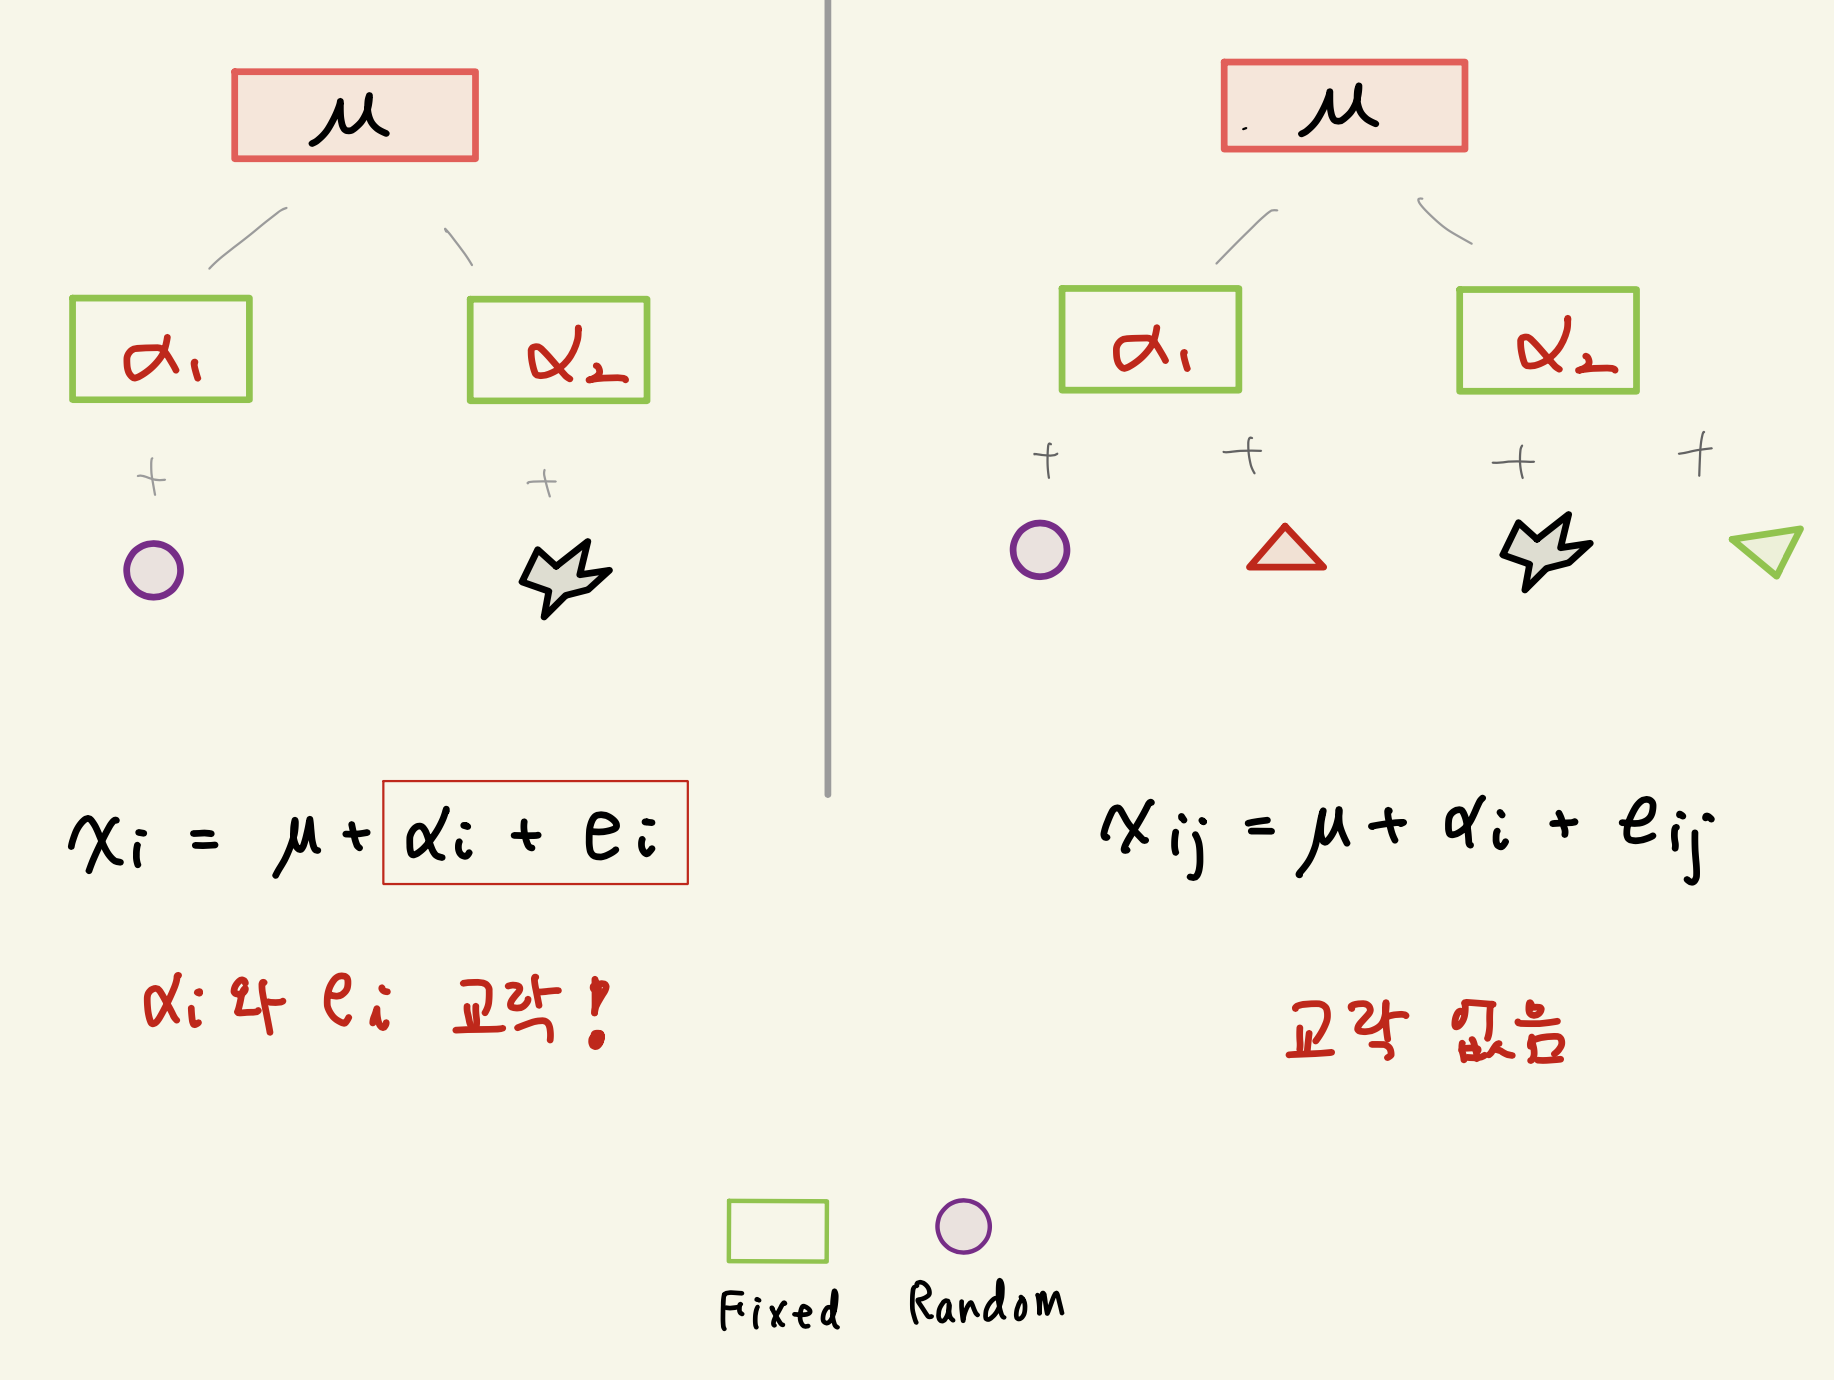
\includegraphics[width=0.7\textwidth,height=\textheight]{confound1.png}
\caption{일원배치: 반복이 없는 경우와 있는 경우}
\end{figure}

\begin{itemize}
\tightlist
\item
  반복이 없는 일원배치
\end{itemize}

위의 그림에서 반복이 없는 일원배치에서는 처리효과와 실험단위(오차항)가 교락되어 구별할 수 없다.

예를 들어 철수에게는 A 약을 처방하고 영이에게는 B 약을 처방한 경우, 만약 철수의 치료 효과가 영이보다 좋으면 A 약의 효과가 더 좋다고 말할 수 있는가? 이런 경우 약의 효과인지 실험 대상인 개인의 특성인지 알 수 없다.

반복이 없는 일원배치에서는 효과의 차이를 알 수 있는 통계량이 두 관측값의 차이 \(x_1 - x_2\) 밖에 없으며 이를 모형식으로 보면 다음과 같다.

\[ x_1 - x_2 = \alpha_1 - \alpha_2 + e_1 - e_2 \]

즉 처리 효과 \(\alpha_i\)와 오차 \(e_i\)의 효과를 분리해야 하는데 사용할 수 있는 통계량이 하나 밖에 없어서 처리효과에 대한 추론이 불가능하다.

여기서 유의할 점은 두 관측값의 차이 \(x_1 - x_2\) 와 평균으로부터 편차 \(x_1 -\bar x\)는 기본적으로 같은 정보를 가진 통계량이다.

\[
x_1 -\bar x = \frac{x_2 - x_1}{2}
\]

\begin{itemize}
\tightlist
\item
  반복이 있는 일원배치
\end{itemize}

반복이 있는 일원배치의 경우 우리는 2개의 편차를 만들 수 있으며 두 편차가 가지고 정보에서 처리 효과에 대한 정보를 분리해 낼수 있다.

\begin{align*}
x_{11} - \bar { \bar x }  & = ( x_{11} - \bar x_{1.}) +  (  {\bar x}_{1.} - \bar { \bar x }) \\
  & = \frac{1}{2} \left [ (-1)x_{12} +(1) x_{11} + (0)x_{21} + (0) x_{22} \right ] \\
   &~ + \frac{1}{4}  \left [ (1)x_{12} +(1) x_{11} + (-1)x_{21} + (-1) x_{22} \right ]  \\ 
  & =  ( e_{11} -  {\bar e}_{1.} ) +  ( [\alpha_1 - \bar \alpha] - [ {\bar e}_{1.} - \bar {\bar e} ])
\end{align*}

반복이 있는 일원배치에서 잔차제곱합 \(MS_E\)는 \(x_{ij} - \bar x_{i.}\)가 지닌 정보, 즉 오차항의 분산에 대한 정보를 가지고 있다.
또한 \(MS_A\)는 \(\bar x_{i.}- \bar { \bar x }\) 가 지닌 정보, 즉 오차항의 분산과 처리 효과의 정보 모두 가지고 있다. 이러한 사실은 각 평균제곱합의 기대값을 보면 알 수 있다.

\[
E (MS_E) = \sigma_E^2,  \quad E(MS_A) = \sigma^2_E + r \frac {\sum_i^a (\alpha_i - \bar \alpha)^2}{a-1}  
\]

따라서 처리효과가 있는지에 대한 검정은 \(MS_E\)와 \(MS_E\)의 비(ratio)를 이용하여 검정한다(F-검정).

\hypertarget{uxc644uxc804-uxb79cuxb364uxd654-uxc774uxc6d0uxbc30uxce58}{%
\subsection{완전 랜덤화 이원배치}\label{uxc644uxc804-uxb79cuxb364uxd654-uxc774uxc6d0uxbc30uxce58}}

이제 이원배치에서 반복이 없는 경우와 있는 경우를 살펴보자.

\hypertarget{uxbc18uxbcf5uxc774-uxc5c6uxb294-uxc774uxc6d0uxbc30uxce58}{%
\subsubsection{반복이 없는 이원배치}\label{uxbc18uxbcf5uxc774-uxc5c6uxb294-uxc774uxc6d0uxbc30uxce58}}

\begin{figure}
\centering
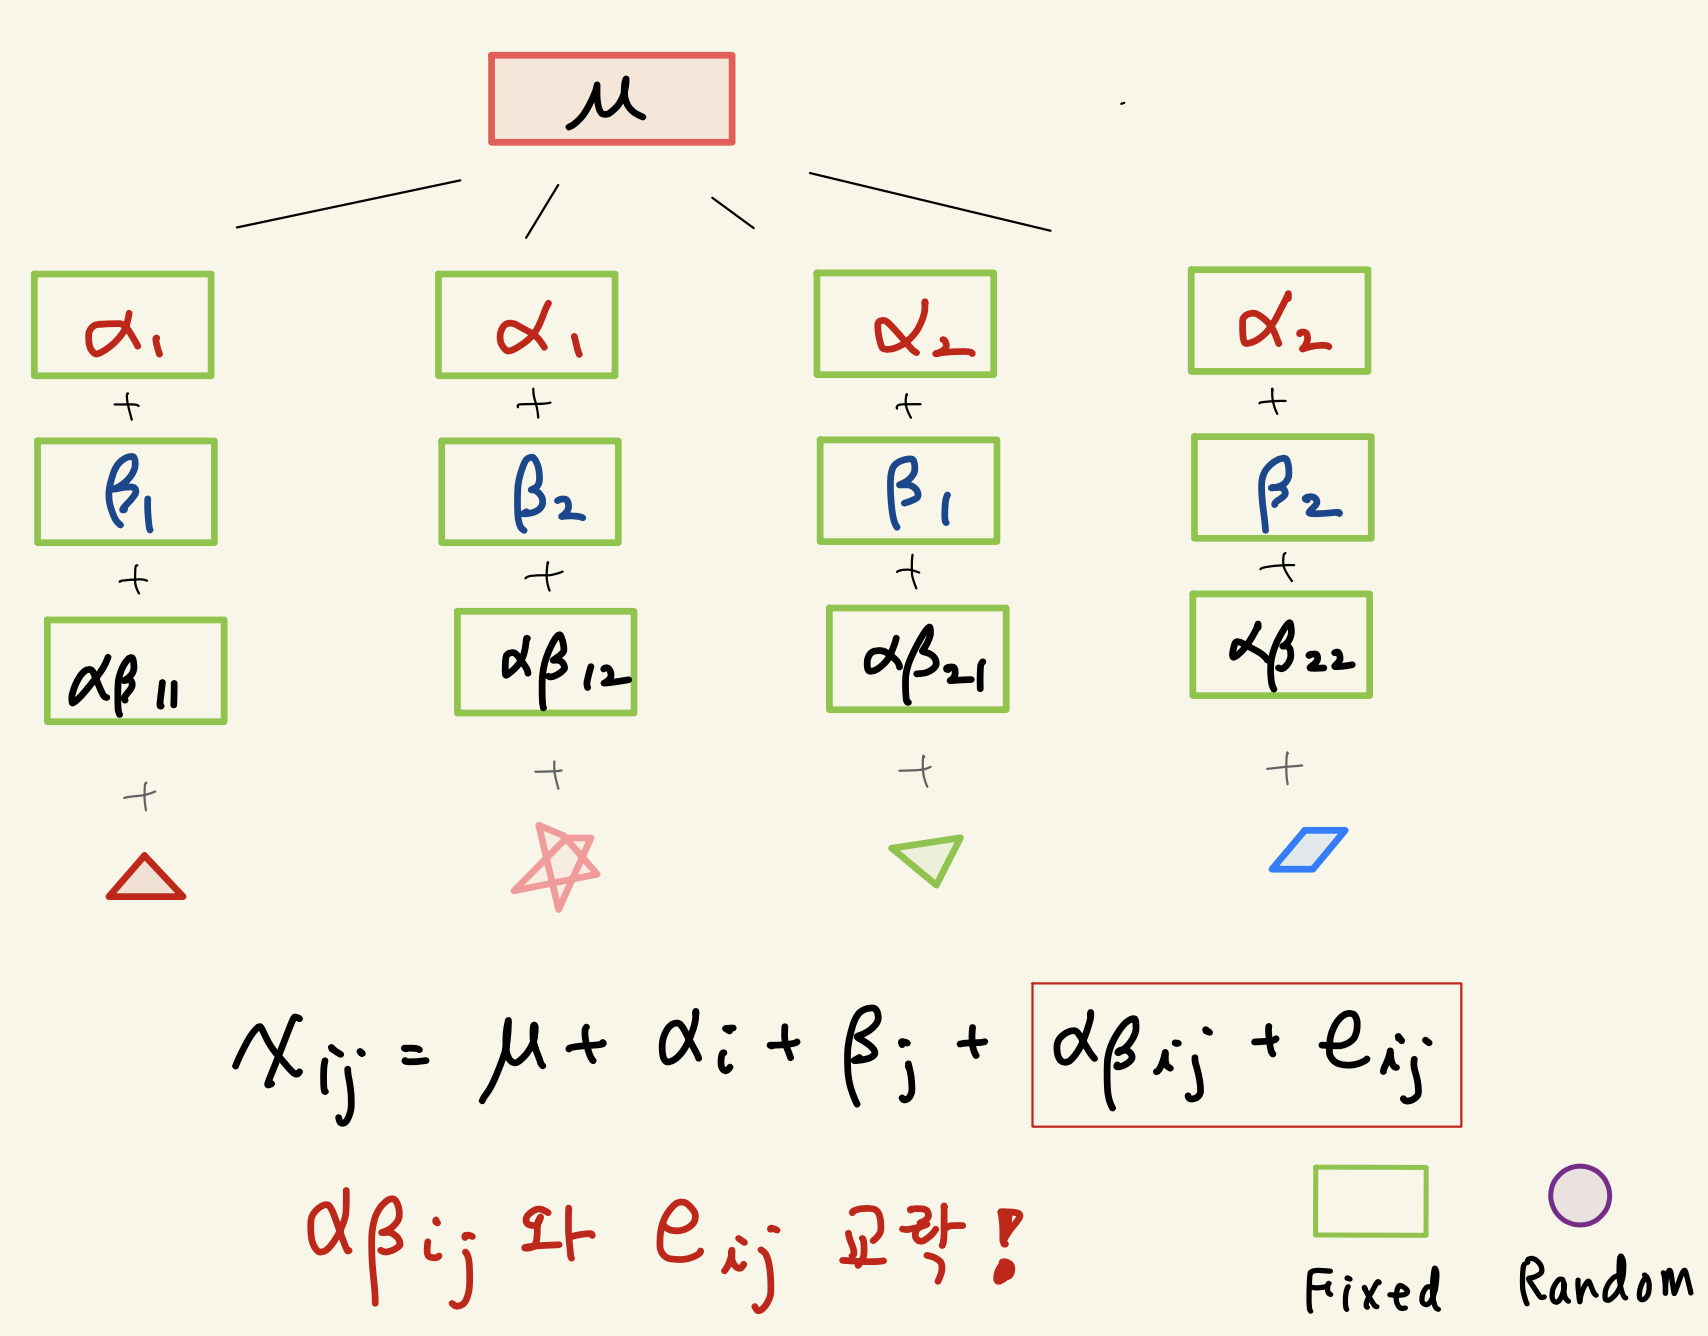
\includegraphics[width=0.7\textwidth,height=\textheight]{confound2.png}
\caption{이원배치: 반복이 없는 경우}
\end{figure}

반복이 없는 이원배치는 관측자료의 편차를 각 효과에 대한 편차들로 다음과 같이 분해할 수 있다.

\[ 
 \underbrace{ ( {x}_{ij} - \bar{\bar {x}} )}_{\text{total deviation}}= \underbrace{( {\bar x}_{i.} - \bar{\bar {x}} ) }_{\text{A effect}} + \underbrace{( {\bar x}_{.j} - \bar{\bar {x}} ) }_{\text{B effect}} + \underbrace{ ( x_{ij} -{\bar x}_{i.} - {\bar x}_{.j} + \bar{\bar {x}}  )}_{\text{(A x B) + residual}} 
\]
위의 분해에서 이원배치 모형식을 이용하여 마지막 항 \(x_{ij} -{\bar x}_{i.} - {\bar x}_{.j} + \bar{\bar {x}}\) 을 모수와 오차로 표현해보면 다음과 같다.

\begin{equation}
x_{ij} -{\bar x}_{i.} - {\bar x}_{.j} + \bar{\bar {x}}  = 
[ (\alpha \beta)_{ij} - \bar {(\alpha \beta)}_{i. } -\bar {(\alpha \beta)}_{.j} + \bar {\bar {(\alpha \beta)}} ]  +
[ e_{ij} - \bar {e}_{i. } -\bar {e}_{.j} + \bar {\bar {e}}]
\label{eq:inter}
\end{equation}

위의 식을 보면 편차 \(x_{ij} -{\bar x}_{i.} - {\bar x}_{.j} + \bar{\bar {x}}\) 는 상호작용에 대한 정보와 오차항의 정보가 섞여 있고
더 이상 분리할 수 없음을 알 수 있다. 따라서 상호작용과 오차항은 교락되어 있다.

\hypertarget{uxbc18uxbcf5uxc774-uxc788uxb294-uxc774uxc6d0uxbc30uxce58}{%
\subsubsection{반복이 있는 이원배치}\label{uxbc18uxbcf5uxc774-uxc788uxb294-uxc774uxc6d0uxbc30uxce58}}

\begin{figure}
\centering
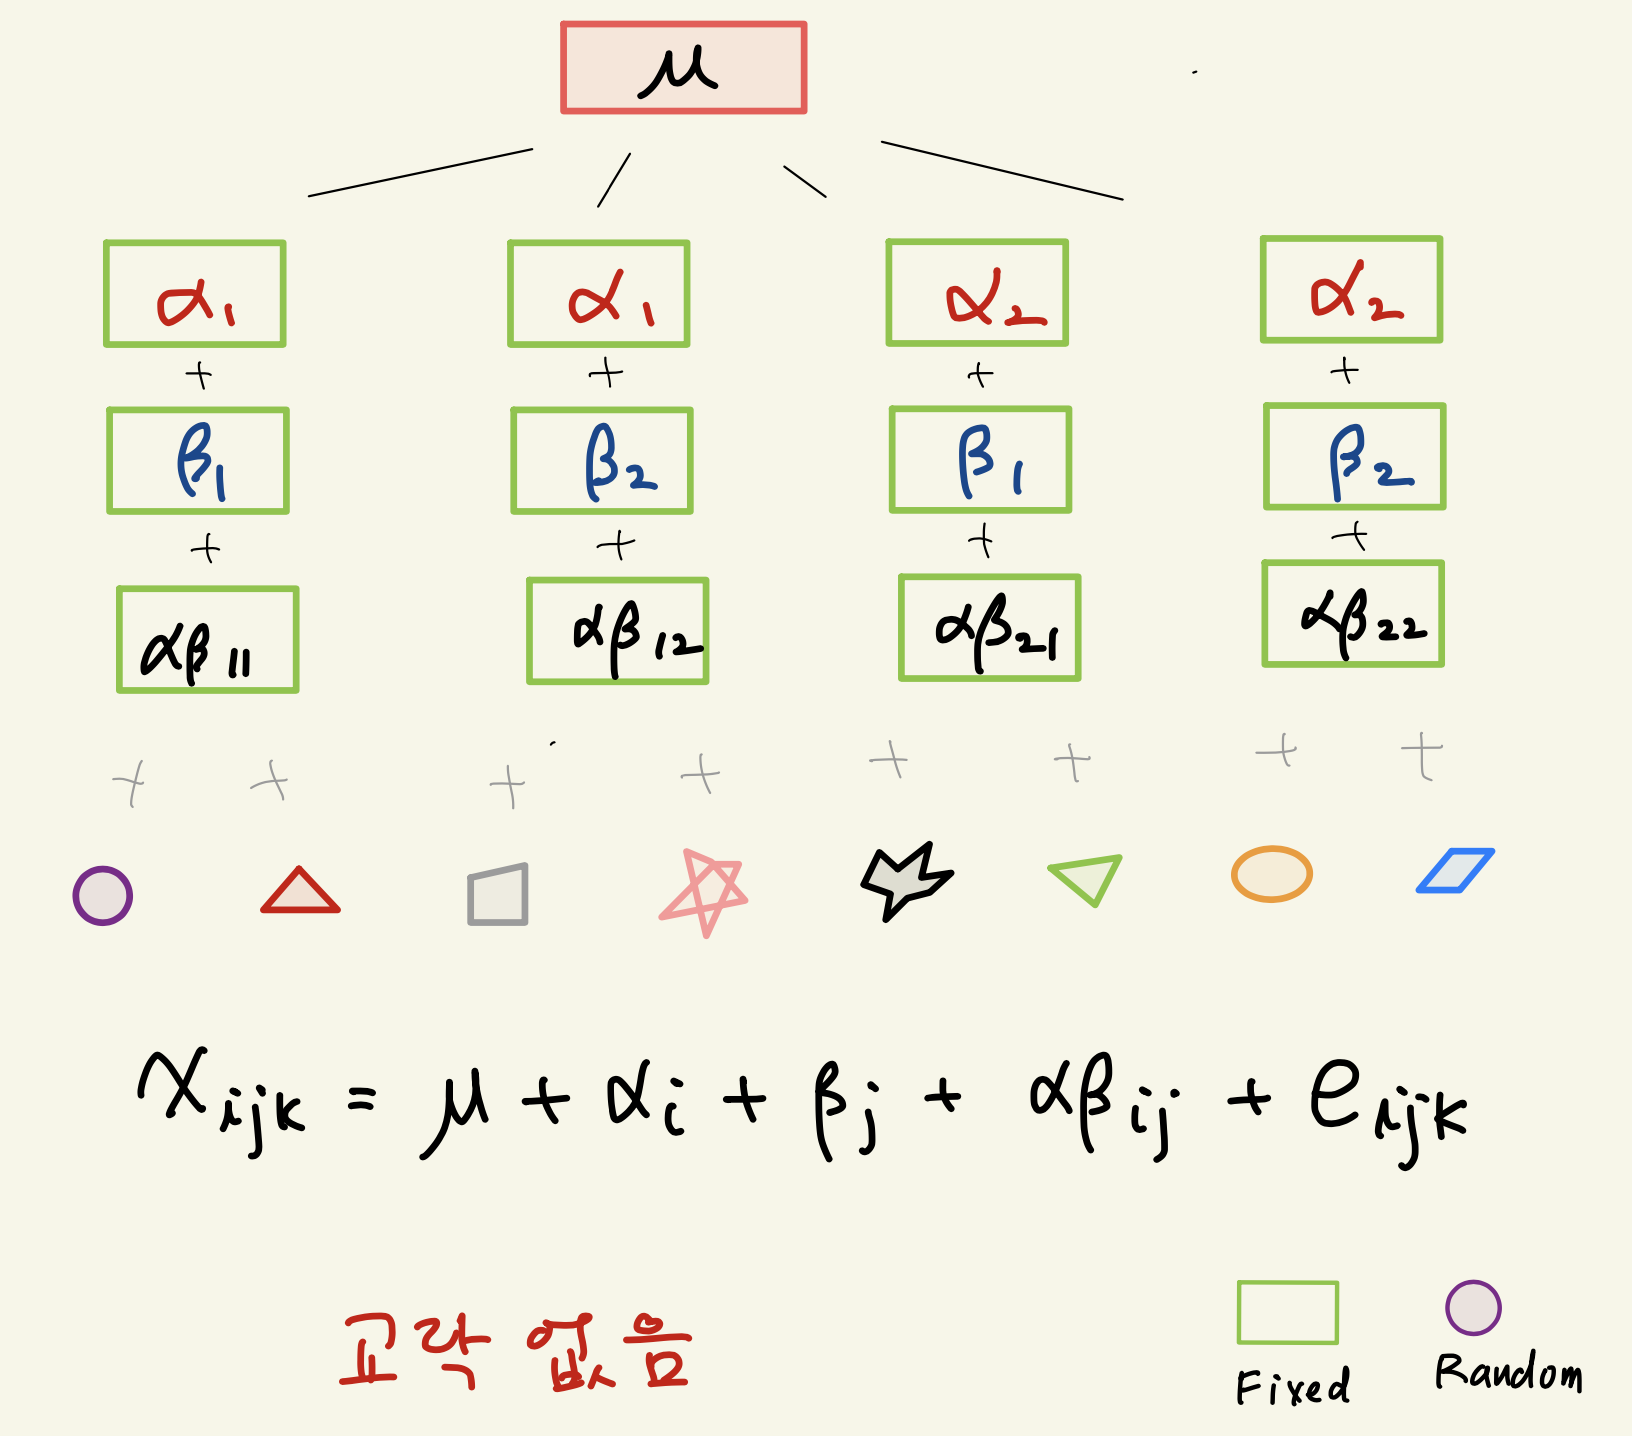
\includegraphics[width=0.7\textwidth,height=\textheight]{confound3.png}
\caption{이원배치: 반복이 있는 경우}
\end{figure}

반복이 있는 이원배치는 관측자료의 편차를 각 효과에 대한 편차들로 다음과 같이 분해할 수 있다. 주목할 점은 반복이 있기 떄문에 반복이 없는 경우보다 하나의 항 \(x_{ijk} - {\bar x}_{ij.}\) 이 추가된다.

\[ 
\underbrace{ (x_{ijk} - \bar{\bar {x}}) }_{\text{total deviation}} = 
\underbrace{( {\bar x}_{i..} - \bar{\bar {x}} ) }_{\text{A effect}} + \underbrace{( {\bar x}_{.j.} - \bar{\bar {x}} ) }_{\text{B effect}} + \underbrace{ ( {\bar x}_{ij.} -{\bar x}_{i..} - {\bar x}_{.j.} + \bar{\bar {x}}  )}_{\text{A x B}} 
+ \underbrace{ ( x_{ijk} - {\bar x}_{ij.} )}_{\text{residual}} 
\]

반복이 있는 이원배치 모형에서 상호작용에 대한 편차는 반복이 없는 경우의 식 \eqref{eq:inter}과 유사하게 다음과 같이 표시할 수 있다.

\[
x_{ij.} -{\bar x}_{i..} - {\bar x}_{..j} + \bar{\bar {x}}  = 
[ (\alpha \beta)_{ij.} - \bar {(\alpha \beta)}_{i. } -\bar {(\alpha \beta)}_{.j} + \bar {\bar {(\alpha \beta)}} ] + 
[ e_{ij.} - \bar {e}_{i.. } -\bar {e}_{.j.} + \bar {\bar {e}}]
\]

또한 잔차에 대한 편차는 다음과 같이 표시된다.

\[
x_{ijk} - {\bar x}_{ij.} = e_{ijk} - \bar {e}_{ij. }
\]
이제 잔차에 대한 편차는 순수허게 오차항만의 정보를 가지고 있고 상호작용에 대한 편차는 상호작용과 오차에 대한 정보를 가지고 있다. 따라서 두 편차로 만든 두 개의 제곱합을 이용하면 상호작용에 대한 효과를 분리해낼 수 있다.

따라서 상호작용 효과가 있는지에 대한 검정은 \(x_{ij.} -{\bar x}_{i..} - {\bar x}_{..j} + \bar{\bar {x}}\) 로 계산된 \(MS_{(A \times B)}\)와 \(x_{ijk} - {\bar x}_{ij.}\) 로 만들어진 \(MS_E\)의 비(ratio)를 이용하여 검정한다(F-검정).

  \bibliography{book.bib,packages.bib}

\end{document}
